\documentclass[10pt]{beamer}

\usepackage[utf8]{vietnam}
\usetheme[secheader]{Boadilla}
\usecolortheme{beaver}
\usefonttheme{professionalfonts}

\usepackage{textpos}
\usepackage{tikz}
\usepackage{graphicx}
\usepackage{xcolor}
\useoutertheme[red,subsection=false]{smoothbars}
%\useoutertheme{smoothtree}
%\logo{
\includegraphics[width=0.7cm]{Figs/fig}\vspace{200pt}}


\definecolor{redd}{RGB}{207,22,40}
\definecolor{yello}{RGB}{243,195,9}

\setbeamercolor*{subitem projected}{fg = yello, bg = redd}%
\setbeamercolor*{structure}{fg = redd}%

\setbeamertemplate{itemize items}{\normalsize$\bullet$} 
\setbeamertemplate{enumerate items}[circle] 
\setbeamertemplate{sections/subsections in toc}[circle]


\pgfdeclareimage[height=\paperheight,width=\paperwidth]{bgimage}{Figs/bg.jpg}
\usebackgroundtemplate{\tikz\node[opacity=0.1,inner sep=0]{\pgfuseimage{bgimage}};}

\title[Nhà quản trị Tim Cook]{Học phần: \textbf{Quản trị học đại cương}}
\subtitle{EM1010 - 116897}
\author[EM1010 - 116897]{\textbf{Chủ đề: Trình bày về nhà quản trị Tim Cook. Qua đó đưa ra khái niệm nhà quản trị, những kỹ năng mà nhà quản trị cần phải có và những tố chất tạo nên một nhà quản trị}}
\institute[Nhóm 6]{\large {Nhóm 6}}
\date{\today}

\beamertemplatetransparentcoveredhigh
\begin{document}

\frame{\titlepage\transsplitverticalout}

\addtobeamertemplate{frametitle}{}{%
\begin{textblock*}{100mm}(.95\textwidth,-0.8cm)

\includegraphics[width=0.7cm]{Figs/fig}
\end{textblock*}}

\begin{frame}
\label{contents}
\transblindshorizontal
\frametitle{\textbf{Nội dung}}
\tableofcontents
\end{frame}

\section{Tìm hiểu về nhà quản trị Tim Cook}

\subsection{Tiểu sử}
\begin{frame}
\transsplitverticalin
\frametitle{Tiểu sử}
\begin{figure}
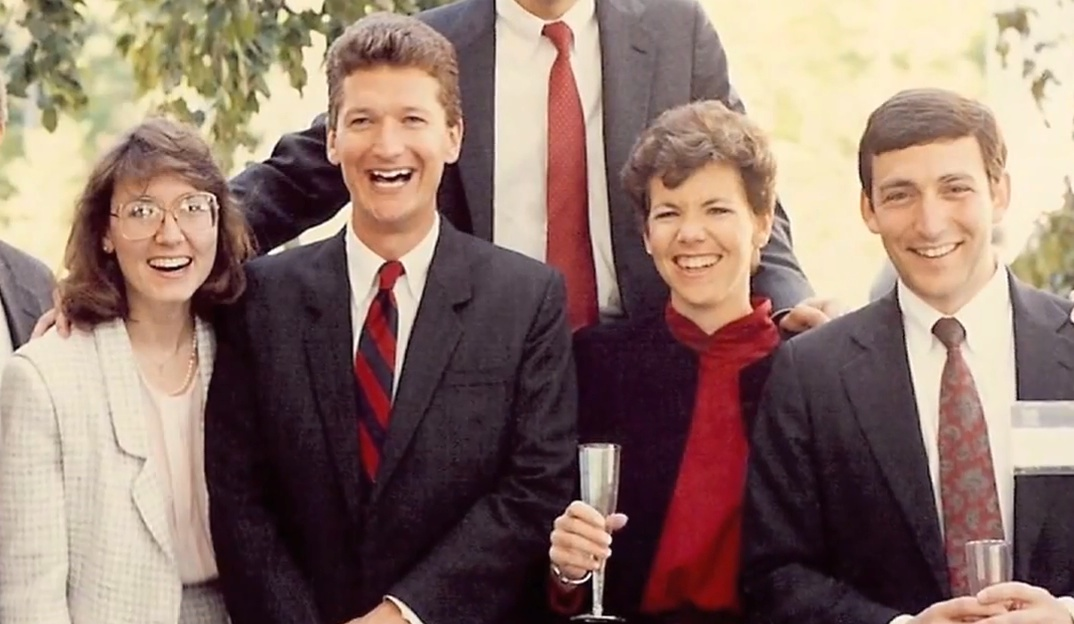
\includegraphics[scale=0.17]{Figs/fig1.jpg}
\caption{Tim Cook cùng bạn bè tại Đại học Auburn}
\end{figure}
\pause
\begin{itemize}
\item Timothy Donald Cook(Tim Cook) sinh ngày 1 tháng 11 năm 1960, lớn lên ở Robertsdale, tiểu bang Alabama, Hoa Kỳ.
\pause
\item Tim Cook tốt nghiệp với bằng cử nhân kỹ sư công nghiệp từ Đại học Auburn năm 1982, bằng Thạc sĩ Quản trị Kinh doanh (MBA) từ Trường kinh doanh Fuqua thuộc Trường Đại học Duke năm 1988.
\end{itemize}



\end{frame}

\subsection{Sự nghiệp}
\begin{frame}
\transsplitverticalout
\frametitle{Sự nghiệp}
\pause
\textbf{Trước khi làm việc tại Apple}
\begin{itemize}
\item Cook đã có kinh nghiệm 12 năm kinh doanh máy tính cá nhân của IBM, cuối cùng đảm nhận vị trí giám đốc của North American Fulfillment.
\item Ông từng là Giám đốc điều hành đại lý bán lẻ máy tính của Intelligent Electronics, Phó chủ tịch của Compaq
%\item Năm 1997 trở thành Phó Chủ tịch mảng dữ liệu doanh nghiệp cho Compaq trong 6 tháng.
\end{itemize}
\pause
\vspace{10pt}
\textbf{Làm việc tại Apple}
\begin{itemize}
%\item Vị trí đầu tiên của ông là phó chủ tịch cấp cao của Worldwide Operations.
\item Bắt đầu từ 2015, Cook đưa ra các quyết định đầu tư \emph{quan trọng} nhưng khá \emph{mạo hiểm}, ảnh hưởng đến tương lai của Apple. Ví dụ hợp đồng với các công ty chuyên sản xuất bộ nhớ flash hay các ổ lưu trữ trên máy tính, từ đó tạo nên những sản phẩm như điện thoại iPhone hay máy tính bảng iPad.
\item Hành động này của Cook đã được công nhận với việc giữ \textit{kiểm soát chi phí}, kết hợp với sự hiểu biết về thiết kế và tiếp thị của công ty, tạo ra \textit{lợi nhuận khổng lồ}.
\end{itemize}
\end{frame}

\begin{frame}
\transblindshorizontal
\frametitle{Sự nghiệp}

%\begin{itemize}
%\item Năm 2011, Hội đồng quản trị của Apple đã phê duyệt đợt nghỉ phép y tế lần thứ ba theo yêu cầu của Jobs - \emph{Nhà sáng lập Apple}. Trong thời gian đó, Cook chịu trách nhiệm cho hầu hết các hoạt động thường ngày của Apple.
%\end{itemize}
\pause
\textbf{Giám đốc điều hành của Apple (2011 - nay)}
\begin{itemize}
\item Ngày 29 tháng 10 năm 2012, Cook thực hiện thay đổi lớn đối với đội ngũ điều hành của công ty.
\item Thay đổi nhân sự của Cook xảy ra sau khi tổng kết doanh thu quý 3, khi doanh thu và lợi nhuận tăng trưởng tăng ít hơn dự đoán.
\item Kể từ khi trở thành CEO, Cook tập trung vào xây dựng một nền văn hóa hài hòa có nghĩa là loại bỏ những người mà Jobs dung thứ và giữ bên mình.
\item Năm 2014, Cook đã gây xôn xao khi ông thách thức các cổ đông ``\emph{rời khỏi tập đoàn}'' nếu họ \emph{không đồng tình} với quan điểm của công ty về sử dụng sản phẩm \emph{thân thiện với môi trường và biến đổi khí hậu}.
\end{itemize}
\end{frame}

\begin{frame}
\transsplitverticalin
\frametitle{Sự nghiệp}
\begin{figure}
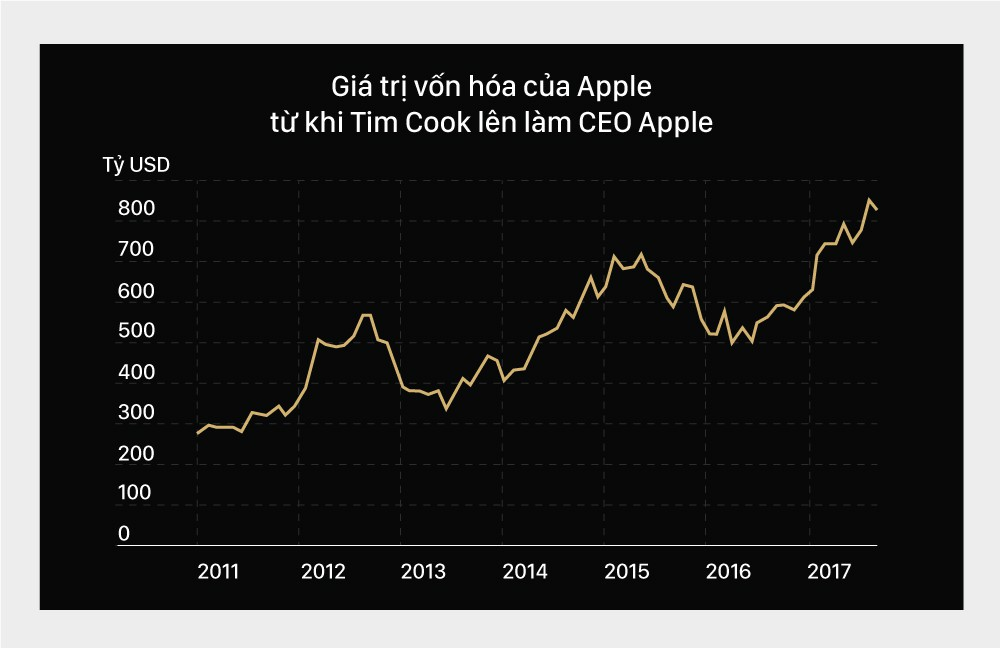
\includegraphics[scale=0.2]{Figs/vonhoa.jpg}
\end{figure}

Ông đã chứng minh cho cả thế giới thấy Apple dưới triều đại của ông thịnh vượng như thế nào với lợi nhuận khủng khiếp. Đến từ những quyết định tưởng như nhỏ nhưng tối ưu lợi nhuận cho hãng, là công ty đầu tiên đạt giá trị trên 800 tỷ USD (Tính đến tháng 1/2020 là 1300 tỷ USD)
\end{frame}

\begin{frame}
\transsplitverticalout
\frametitle{Sự nghiệp}

\begin{figure}
\centering
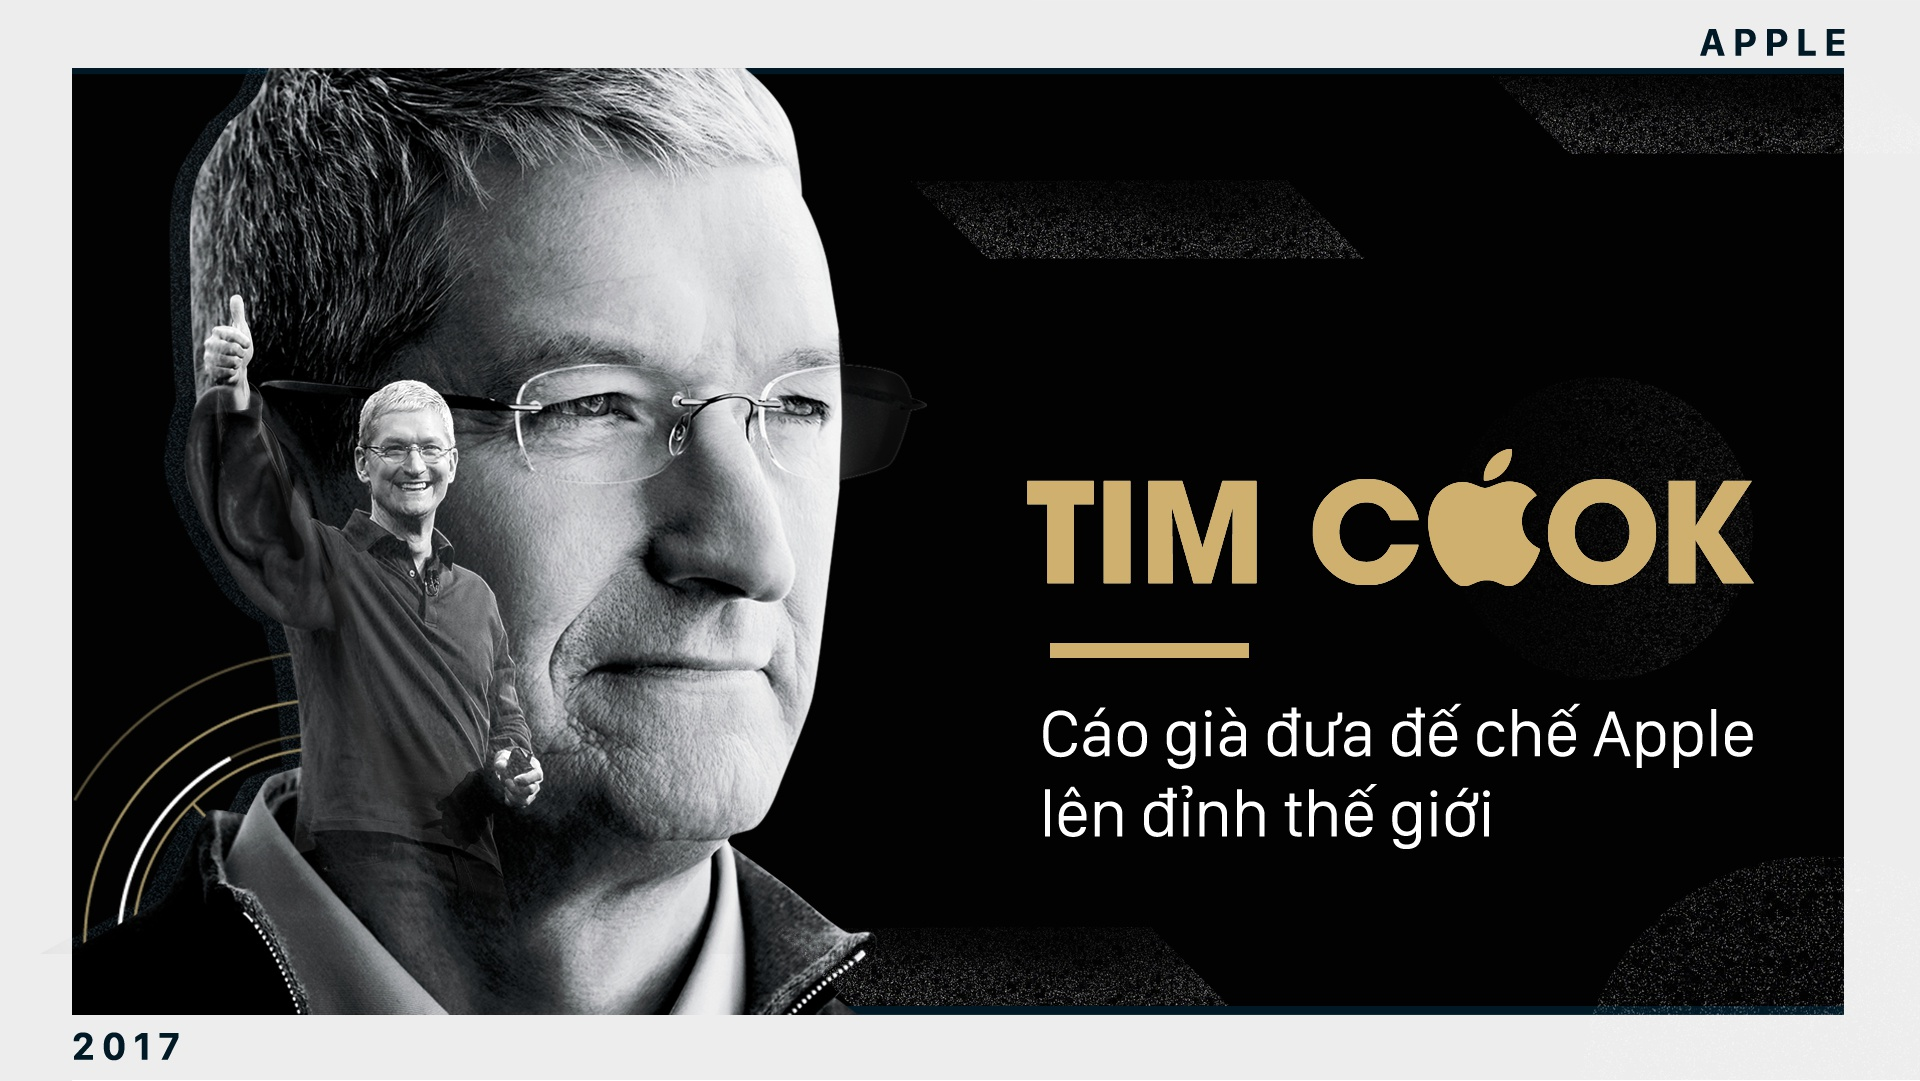
\includegraphics[scale=0.15]{Figs/timcook.jpg}

Source: Internet
\end{figure}
\end{frame}



\section{Khái niệm nhà quản trị}

\subsection{Định nghĩa quản trị}
\begin{frame}{Khái niệm nhà quản trị}
\transsplitverticalout
%\frametitle{Định nghĩa}
\pause
Thuật ngữ \emph{quản trị} được giải thích bằng nhiều cách khác nhau và có thể nói là chưa có một định nghĩa nào được tất cả mọi người chấp nhận hoàn toàn.
\pause
\begin{itemize}
\item Theo Mary Parkr Follett: “Quản trị là nghệ thuật đạt được mục đích thông qua người khác”.
\pause
\item Theo James Stoner và Stephen Robbins thì: “Quản trị là tiến trình hoạch định, tổ chức, lãnh đạo và kiểm soát những hoạt động của các thành viên trong tổ chức và sử dụng tất cả các nguồn lực khác của tổ chức nhằm đạt được mục tiêu đã đề ra”.
\end{itemize}

\begin{figure}

\includegraphics[scale=0.14]{Figs/fig3}
\end{figure}

\end{frame}

\subsection{Quản trị học mang tính khoa học hay nghệ thuật}


\begin{frame}
\transblindshorizontal
\frametitle{Quản trị học mang tính khoa học hay nghệ thuật?}
\begin{columns}

\column{0.45\textwidth}

\includegraphics[scale=0.3]{Figs/fig4.png}
\pause
\column{0.6\textwidth}
\textbf{Quản trị mang tính khoa học}: Quản trị là một khoa học vì nó có đối tượng nghiên cứu cụ thể, có phương pháp phân tích và có lý thuyết xuất phát từ các nghiên cứu.\\
\pause
\vspace{10pt}
\textbf{Quản trị là một nghệ thuật}:
\begin{itemize}
\item Quản trị là quá trình làm việc với con người và thông qua con người.
\item Quản trị được học thông qua kinh nghiệm thực tiễn, mà kinh nghiệm thực tiễn lại được hoàn thiện bởi những con người có tài năng tương ứng.
\end{itemize}

\end{columns}


\end{frame}


\subsection{Phân biệt quản trị, quản lý và lãnh đạo}

\begin{frame}
\transsplitverticalin
\frametitle{Phân biệt quản trị, quản lý và lãnh đạo}
\pause
\textbf{Quản trị} về bản chất là quản lý, nhưng ở tầm vĩ mô hơn, tập trung vào các nguyên tắc, quy tắc, luật lệ, chuẩn mực vận hành, ví dụ các nguyên tắc quản trị công ty (\emph{corporate governance principles}, viết tắt là CGP).\\
\pause
\vspace{10pt}
\textbf{Quản lý}(corporate management) tập trung vào công tác quản lý (chiến lược, mô hình, cơ cấu, marketing, thương hiệu, bán hàng, tài chính, kế toán, nguồn nhân lực, sản xuất, cung ứng, quản lý chất lượng…) và hoạt động điều hành hàng ngày (daily operations).\\
\pause
\vspace{10pt}
\textbf{Lãnh đạo} là chỉ ra những việc đúng để làm (do the right things), còn quản trị và quản lý là làm đúng cách, đúng phương pháp. Lãnh đạo tập trung vào tầm nhìn, định hướng, sức thu hút, ảnh hưởng, nghệ thuật dùng người (đúng người, đúng việc, đúng thời điểm, đúng nơi…), đạo đức, uy tín, nhân cách người lãnh đạo…\\

\pause
%\begin{block}{Cần hiểu rằng}
%Cả quản trị lẫn quản lý đều cần đến nguyên tắc, quy tắc, luật lệ, quy chế, phương pháp kiểm soát…, và đều là những công việc mang tính khoa học (science). Trong khi đó lãnh đạo (leadership) lại thiên về nghệ thuật (art). Tất nhiên, nhà quản trị hay nhà quản lý đều ít nhiều phải có \textit{tố chất lãnh đạo}, và phải có \textit{nghệ thuật lãnh đạo}.
%\end{block}

\end{frame}

\section{Những kỹ năng mà nhà quản trị cần có}

\subsection{Khái niệm về kỹ năng quản trị}
\begin{frame}
\transsplitverticalout
\frametitle{Khái niệm về kỹ năng quản trị}

\emph{Kỹ năng quản trị} là những khả năng, kinh nghiệm, kỹ xảo và mức độ thành thạo trong việc thực hiện công việc trong các lĩnh vực, chức năng quản trị doanh nghiệp, trong điều kiện và hoàn cảnh nhất định.
\begin{figure}
\centering

\includegraphics[scale=0.09]{Figs/fig5}
\end{figure}

\end{frame}


\subsection{Các kỹ năng nhà quản trị cần phải có}
\begin{frame}
\transblindshorizontal
\pause
\frametitle{Các kỹ năng nhà quản trị cần phải có}
\textbf{Kỹ năng kỹ thuật}: Là trình độ chuyên môn nghiệp vụ của nhà quản trị, bao hàm sự hiểu biết và thành thạo về một loại hình hoạt động đặc biệt, nhất là loại hình hoạt động có liên quan đến phương pháp, các chu trình, các thủ tục hay các kỹ thuật của lĩnh vực, chức năng của nhà quản trị đang đảm nhận. Là kỹ năng quan trọng của một nhà \underline{\emph{quản trị cấp cơ sở}}. 
\pause

\vspace{10pt}
\textbf{Kỹ năng nhân sự}: Là khả năng cùng làm việc, động viên, điều khiển con người và tập thể trong doanh nghiệp, dù những người đó là thuộc cấp, đồng nghiệp ngang hàng hay cấp trên. Là kỹ năng quan trọng của một nhà \underline{\emph{quản trị cấp trung}}. 
\pause

\vspace{10pt}
\textbf{Kỹ năng nhận thức,tư duy}: Là khả năng tư duy hệ thống, biết phân tích mối liên hệ giữa các vấn đề một cách logic. Đây là một kỹ năng rất khó và đặc biệt hiểu rõ mức độ phức tạp của môi trường và biết cách giảm thiểu sự phức tạp đó xuống một mức có thể đối phó được. Là kỹ năng quan trọng của một nhà \underline{\emph{quản trị cấp cao}}.
\end{frame}

\begin{frame}{Các kỹ năng nhà quản trị cần phải có}
\transsplitverticalin
\centering
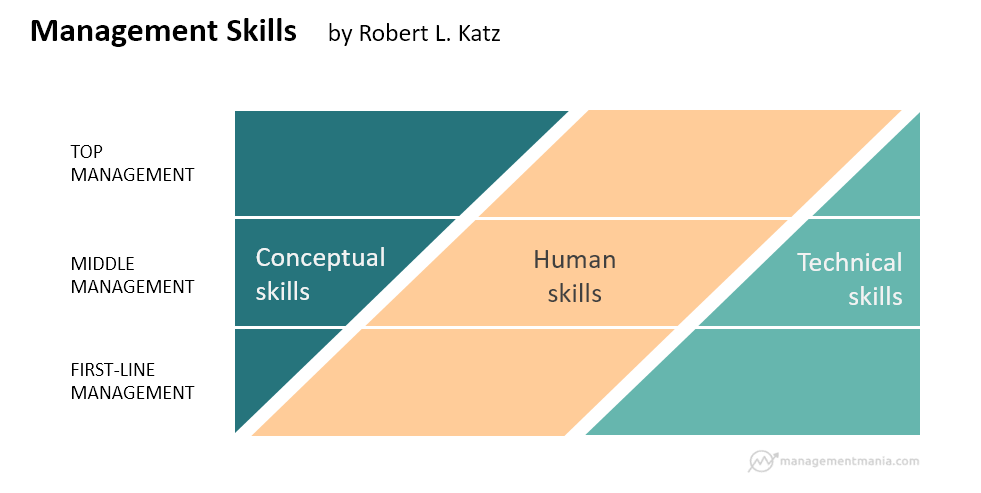
\includegraphics[scale=0.4]{Figs/fig6}
\end{frame}

\subsection{Tim Cook: Tổng giám đốc công ty Apple.Inc và những kỹ năng quản trị}
\begin{frame}
\transsplitverticalout
\frametitle{Tim Cook - Những kỹ năng quản tị}
\pause
\textbf{Kỹ năng kỹ thuật}:
Trước khi làm việc cho Apple, Tim Cook có 12 năm làm việc cho IBM, ông đã trực tiếp làm việc với dây chuyền sản xuất, bắt đầu từ những khâu cơ bản nhất như đảm bảo nhà máy đủ linh kiện để lắp ráp.
\pause

\vspace{15pt}
\textbf{Kỹ năng nhân sự}:
\begin{itemize}
\item Vị CEO này luôn biết san sẻ công việc cho những người xung quanh cũng như cho họ quyền tự quyết.
Đó là một việc thể hiện sự tin tưởng đồng đội tuyệt đối và giúp \emph{Táo khuyết} có được vị trí hàng đầu như ngày hôm nay.
\item Tim Cook đề cao văn hóa tôn trọng lẫn nhau giữa các nhà quản trị và nhân viên của Apple. Đặc biệt là phương châm làm việc “không cố quá khả năng” luôn khiến nhân viên được làm việc trong một môi trường dễ thở. 
\end{itemize}
\end{frame}

\begin{frame}
\transblindshorizontal
\frametitle{Tim Cook - Những kỹ năng quản tị}
\pause
\textbf{Kỹ năng nhận thức hay tư duy}:
\emph{Triều đại} của Apple dưới thời Tim Cook bắt đầu không hề suôn sẻ.

Ông đã lèo lái khéo léo để một mặt trung thành với những nét tạo nên sự độc đáo của Apple, một mặt bổ sung các giá trị theo cách của riêng mình, những điều chính Steve Jobs cũng chưa làm được.
\begin{figure}
\centering

\includegraphics[scale=0.1]{Figs/fig7}
%\caption{\emph{The metaphor} Tim Cook uses means you should not let a barrier stop you. One way is to climb over it}
\end{figure}
\end{frame}

\begin{frame}
\transsplitverticalin
\frametitle{Bí quyết nào khiến Tim Cook lọt vào top những nhà quản trị có tầm ảnh hưởng trên thế giới?}
\pause
\textbf{Coi trọng sự đa dạng}: Sự đa dạng về chuyên môn giữa các nhân viên có thể làm tăng doanh thu của công ty. Ý tưởng ẩn sau triết lý này là mọi người có thể có những kinh nghiệm khác nhau và công ty có thể tận dụng lợi thế từ các kinh nghiệm quý báu của mỗi cá thể để đạt được thành công.
\pause

\vspace{10pt}
\textbf{Sự minh bạch là chìa khóa}: Với những lời chỉ trích nặng nề về tiêu chuẩn làm việc của nhân viên Apple, Cook đã công khai cho cả thế giới biết về cách hoạt động của Apple. Bằng cách này, ông không chỉ tạo ra thiện chí trong văn phòng mà còn đặt tiêu chuẩn cho những nhà máy khác.
\pause

\vspace{10pt}
\textbf{Đọc thư của khách hàng}: Tim Cook, người đứng đầu một công ty giá trị nhất thế giới, vẫn dành thời gian thăm các cửa hàng của công ty và đọc thư của khách hàng. 
\end{frame}

\begin{frame}
\transsplitverticalout
\frametitle{Bí quyết nào khiến Tim Cook lọt vào top những nhà quản trị có tầm ảnh hưởng trên thế giới?}
\pause
\textbf{Chỉ làm được một vài điều tuyệt vời}: Hãy xem xét đến quy mô của Apple! Công ty chỉ tạo ra một vài sản phẩm. Ông chia sẻ: “\emph{Nếu bạn thực sự quan tâm đến Apple, bạn sẽ thấy chúng tôi có 4 loại Ipods. Chúng tôi có hai loại Iphone chính. Chúng tôi có hai loại Ipad và một vài máy tính Macs.  Và đó là tất cả}”. Vấn đề nằm ở chỗ: tập trung vào việc bạn làm tốt nhất và làm nó trong hết khả năng của bạn.
\begin{figure}
\centering
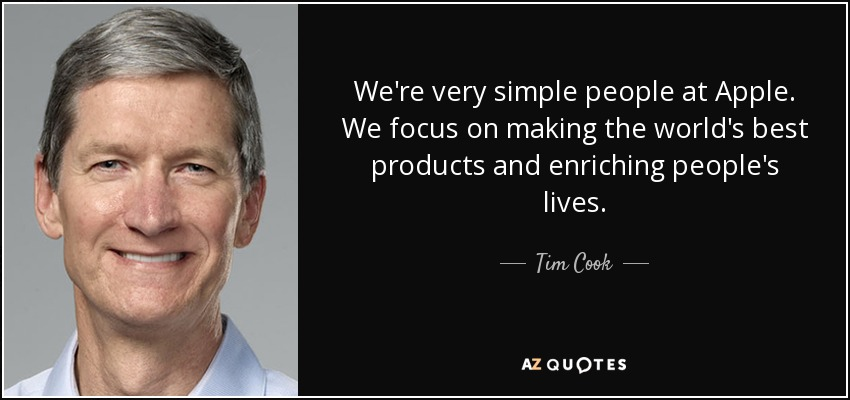
\includegraphics[scale=0.25]{Figs/fig8}
\end{figure}

\end{frame}





\section{Những tố chất tạo nên một nhà quản trị}
\begin{frame}
\transblindshorizontal
\frametitle{Những tố chất tạo nên một Nhà Quản Trị(NQT)}
\pause
\begin{itemize}
\item[1.]\textbf{Tố chất học hỏi}: Không phải ai cũng có thể làm NQT được, và cách đơn giản nhất để thành 1 NQT là học hỏi từ những NQT khác có kinh nghiệm hơn mình.
\pause
\item[2.]\textbf{Tính liêm chính}: Các nhân viên muốn các NQT của họ trung thực, công bằng, vô tư, thẳng thắn và trao cho mọi người những cơ hội ngang nhau, bao gồm sự thăng tiến, công việc và đào tạo... Khi NQT hành động một cách liêm chính, các nhân viên sẽ đáp lại như vậy và họ sẽ trung thành hơn với NQT cũng như tổ chức.
\pause
\item[3.]\textbf{Truyền cảm hứng đối với công việc theo nhóm}: Việc tạo ra các nhóm có năng lượng và nỗ lực sẽ thực sự giúp hoàn thành mọi việc, giúp  thời gian xao lãng  giảm đi, và sự gắn kết, tự giác,năng suất sẽ tăng lên.
\pause
\item[4.]\textbf{Nhà cải cách}: NQT cần có những ý tưởng mới,thử những thứ mới, liên tục dự đoán những cuộc cạnh tranh với những tổ chức khác.
\pause
\item[5.]\textbf{Sẵn sàng chấp nhận thất bại}: Mọi người thường không muốn thất bại, nhưng sẵn sàng thất bại làm cho NQT học được nhiều bài học quý giá từ thất bại, tiến xa hơn về giới hạn và khả năng.
\pause
\item[6.]\textbf{Có niềm tin, hy vọng lớn}: hầu hết NQT đều có khả năng lớn hơn và có thể làm được những điều lớn hơn mà họ nghĩ.
\end{itemize}
\end{frame}
    
\section*{End}
\begin{frame}
\transsplitverticalin
\centering
\begin{tabular}{|c||c|}
\hline 
\textbf{Thành viên} & \textbf{MSSV} \\ 
\hline 
Nguyễn Ngọc Nam & 20171573 \\ 
\hline 
Lê Thị Cẩm Ly & 20174911 \\ 
\hline 
Nguyễn Văn Quang & 20174138 \\ 
\hline 
Nguyễn Trung Kiên  & 20174000 \\ 
\hline 
Nguyễn Thị Thanh Trà  & 20175259 \\ 
\hline 
Phan Trang Nhung  & 20175046 \\ 
\hline 
Nguyễn Trần Thức  & \textit{20185483} \\ 
\hline 
Đỗ Đức Chung & 20171019 \\ 
\hline 
Vũ Đăng Chiến  & 20172432 \\ 
\hline 
Cao Ngọc Đông 
(Nhóm Trưởng)
 & 20161020 \\ 
\hline 
\end{tabular}

\hyperlink{contents}{\beamerbutton{Contents page}}
\end{frame}

\begin{frame}
\transsplitverticalout
\centering
{\fontsize{40}{50} \textcolor{red}{\textbf{Thank You!}}}
\end{frame}


\end{document}